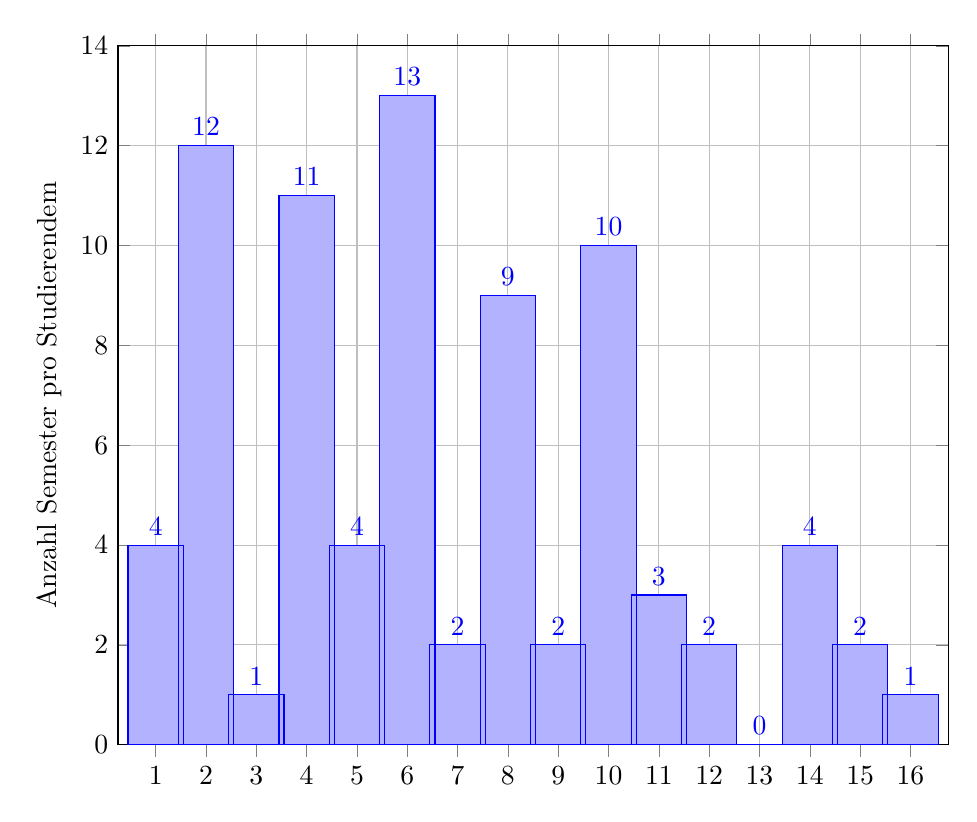
\begin{tikzpicture}
    \begin{axis}[
        x tick label style={
            /pgf/number format/1000 sep=},
        ylabel=Anzahl Semester pro Studierendem,
        enlarge x limits=0.05,
        ymax=14,
        ymin=0,
        ybar,
        bar width=20pt,
        xtick=data,
        xticklabels={1,2,3,4,5,6,7,8,9,10,11,12,13,14,15,16}, 
        width=\linewidth,
        nodes near coords,
        grid=major,
    ]
    
    \addplot coordinates {(1,4) (2,12) (3,1) (4,11) (5,4) (6,13) (7,2) (8,9) (9,2)
    (10,10) (11,3) (12,2) (13,0) (14,4) (15,2) (16,1)};
    \end{axis}
\end{tikzpicture}